% Test fixture: a line chart in pgfplots' default style (grid on both axes, legend box, default markers, a
% dashed data line). Input for the "unify three existing figures" task; the data must survive unchanged.
\documentclass[border=2pt]{standalone}
\usepackage{pgfplots}
\pgfplotsset{compat=1.18}
\begin{document}
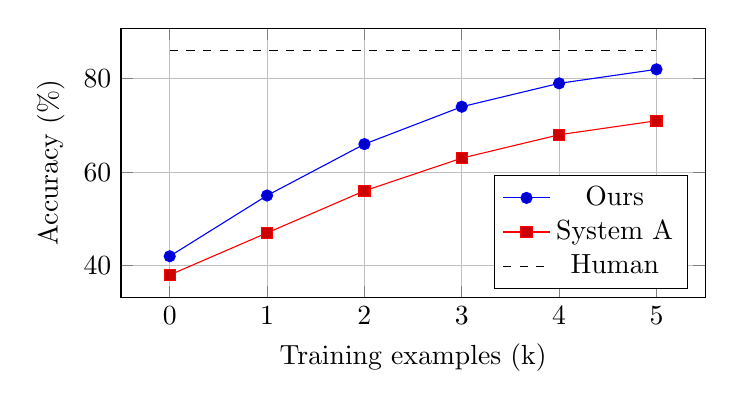
\begin{tikzpicture}
\begin{axis}[width=9cm, height=5cm, xlabel={Training examples (k)}, ylabel={Accuracy (\%)}, grid=both,
  legend pos=south east]
\addplot coordinates {(0,42) (1,55) (2,66) (3,74) (4,79) (5,82)};
\addplot coordinates {(0,38) (1,47) (2,56) (3,63) (4,68) (5,71)};
\addplot[dashed] coordinates {(0,86) (5,86)};
\legend{Ours, System A, Human}
\end{axis}
\end{tikzpicture}
\end{document}
